\section{Methodology}
\label{sec:method}

CodeGraph separates repository retrieval into two explicit responsibilities: lexical signals identify plausible entry points into the codebase, while structural propagation computes the final ranking over reachable code entities. This division of labor is central to the method. Natural-language issue text is used only to place initial probability mass, whereas the ranking itself is determined by repository structure, making retrieval reproducible, interpretable, and aligned with execution semantics. CodeGraph separates computation into two stages: the Indexing Phase constructs the repository graph once, and the Retrieval Phase performs seed selection, graph propagation, and ranking for each query.

\subsection{Seed Selection}

Personalized PageRank requires a set of starting nodes. Seed selection translates the natural-language task description into a personalization vector: a probability distribution determining where the random walk restarts.

CodeGraph constructs this vector from three complementary signals:
\begin{enumerate}
    \item \textbf{Entity match:} Entity match identifies explicit code-like mentions in the task description, including CamelCase and snake\_case identifiers, and maps them directly to nodes in the graph vocabulary. This signal captures cases where the issue text already names a relevant program entity, but it is moderated with inverse-document-frequency (IDF) scaling so that highly ambiguous identifiers, such as common verbs or generic class names, do not dominate the personalization vector.
    \item \textbf{BM25 keyword search:} BM25 keyword search broadens coverage when the issue description does not contain an exact identifier match. Each entity is indexed by its short name, qualified name, file path, and docstring content, allowing lexical relevance to be estimated over multiple views of the same code object. To reduce vocabulary mismatch, compound tokenization splits identifiers at CamelCase boundaries and underscores, so abstract phrases such as ``SQL compilation'' can still recover composite names such as \texttt{SQLCompiler}.
    \item \textbf{Issue path hint:} Issue path hints exploit references to directory names or file names that appear directly in the task description. When such fragments are present, they are mapped to entities under the corresponding repository path, allowing the seed set to be biased toward the relevant module even when the issue text does not explicitly name the final target entity.
\end{enumerate}

These signals are merged to form a robust starting distribution that does not rely exclusively on perfect entity resolution. For example, an issue may mention ``SQL compilation'' without naming the exact implementation file. Compound tokenization allows this phrase to match identifiers such as \texttt{SQLCompiler}, path hints can bias the search toward the relevant module, and the resulting seed set gives Personalized PageRank a structurally meaningful region from which to begin propagation.

\subsection{IDF-Based Edge Reweighting}

Uniform graph traversal assumes every structural connection contributes equally to relevance. In practice, however, some connections point to highly specific domain logic, while others point to generic utility nodes (e.g., global loggers or base classes) reused across large parts of the repository.

To attenuate the influence of generic hubs, CodeGraph assigns each edge a weight inversely proportional to the in-degree of its target node: 
\begin{equation}
    w(e) = \frac{1}{\log_2(\operatorname{in\_degree}(v) + 2)}
    \label{eq:idf-weight}
\end{equation}
This logarithmic penalty steers probability mass away from ubiquitous hubs, ensuring that relevance is propagated primarily along domain-specific pathways. \Cref{fig:idf-reweighting} illustrates this intuition.

\begin{figure}[htbp]
    \centering
    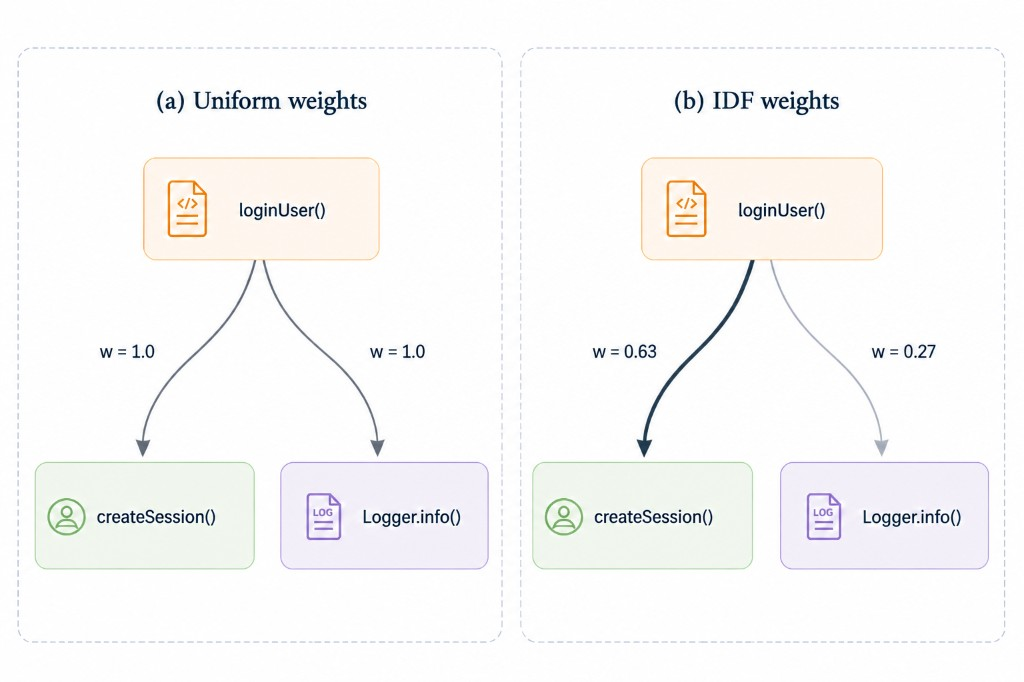
\includegraphics[width=\linewidth]{assets/idf_reweighting.png}
    \caption{IDF edge reweighting. Panel (a) uses uniform weights, diluting relevance. Panel (b) attenuates the weight toward the high in-degree hub, keeping relevance mass on the domain-specific callee.}
    \label{fig:idf-reweighting}
\end{figure}

\subsection{Personalized PageRank Propagation}

With the seed personalization vector $\vec{s}$ and the edge weights $w(e)$ defined, relevance is propagated through the graph using Personalized PageRank (PPR) \cite{jeh2003ppr}. The stationary relevance vector $\vec{r}$ is computed as the solution to:
\begin{equation}
    \vec{r} = (1 - d) \vec{s} + d P^T \vec{r}
    \label{eq:ppr}
\end{equation}
where $d \in (0,1)$ is the damping factor (set to $0.70$), and $P$ is the transition probability matrix. The transition probability from node $u$ to node $v$ is normalized over outgoing edges using the IDF-reweighted values:
\begin{equation}
    P_{uv} = \frac{w(u, v)}{\sum_{(u, k) \in E} w(u, k)}
    \label{eq:transition}
\end{equation}
We compute Personalized PageRank over an undirected projection of the property graph, allowing relevance mass to diffuse both upstream (from callees to callers) and downstream (from callers to callees). This bidirectional propagation is intentional: an issue may describe a callee, a caller, or a related imported component, so retrieval must move in both directions across the dependency graph to recover the correct structural neighborhood. The resulting vector $\vec{r}$ provides a topologically anchored relevance score for every code entity in the repository.

\subsection{Methodological Commitments}

CodeGraph is defined not only by its use of Personalized PageRank, but by four methodological commitments that shape how relevance is represented and propagated through the repository graph.

\textbf{Coarse-Grained Entity Granularity:} The graph schema restricts nodes strictly to files, classes, functions, and methods. CodeGraph explicitly avoids line-level resolution or full Abstract Syntax Tree (AST) ingestion. While ASTs capture complete syntactic correctness, their overwhelming density dilutes retrieval probability mass. The chosen four-entity model provides the exact abstraction layer through which developers typically organize, modularize, and reference code, maintaining a graph size that is efficient for matrix operations.

\textbf{Precision Over Noisy Connectivity:} During graph construction, we resolve calls conservatively. If a function call site is ambiguous and cannot be resolved to a definitive definition within the codebase, CodeGraph omits the edge entirely. This choice favors precision over recall in the graph topology itself: it is safer to miss an implicit connection than to inject false structural pathways that would misdirect the PageRank random walk. 

\textbf{Explicit Dependencies Over Proximity Heuristics:} We restrict edges strictly to syntactic dependencies (\texttt{CALLS}, \texttt{IMPORTS}, \texttt{CONTAINS}, \texttt{INHERITS\_FROM}). We do not use directory-proximity heuristics (e.g., connecting all files in the same folder), as adding proximity edges creates dense subgraphs that indiscriminately diffuse relevance. CodeGraph's retrieval fidelity is built on the premise that execution paths matter more than file system locality.

\textbf{Uniform Restart as a Robustness Mechanism:} A critical algorithmic decision is the use of a uniform restart distribution over the selected seeds, rather than weighting restarts by lexical confidence scores. In software repositories, a highly confident lexical match is often an ambiguous, common identifier (e.g., a generic \texttt{Manager} class). Weighting by confidence amplifies these false positives. Uniform restart is a robustness decision under noisy seed conditions: by giving every extracted seed an equal share of the initial mass, CodeGraph allows the graph topology to arbitrate. Correct seeds that share structural paths compound their mass cooperatively, while isolated incorrect seeds dissipate their relevance into uncoordinated neighborhoods. Taken together, these design choices define CodeGraph as a deterministic repository-level retrieval system in which lexical signals identify entry points and graph propagation determines the final ranking.
